\indent
\indent
In this section, we describe how we develop the project, we set our basis on the start, and them follow them during the development of the project. 

The section is divided in Back-end and Front-End because there where slightly different approaches in the developing process.
\section{Back-End}
Jose I. Retamal
\vskip 0.1in
\indent
\indent
Most successful software projects are developed using some agile methodology\cite{agilemanifesto}. There is a reason for this and is because the software is an intellectual product that needs to adapt to change on requirements, libraries, and hardware. This constant change required adaptative and iterative approaches to develop.

We adapted some of the agile principles to our project \cite{agilemanifesto}:
\begin{itemize}
	\item Continuous delivery. The application is tested at all stages, and we keep a working application all the time.
	\item Adapt to changes at any stage. Even if we started with a design and chose the technologies to be use, they can change at any stage. 
   	\item 	Work together with all participants. We continuously meet with all people involved in the project, check the stage of the project, and check if there is anything that needs to change.
	\item	Self-motivation. There is a personal interest in the project to all participants.
	\item	Working software is the measure of the stage of the project. What is done and working in the software is the main reference point on at what stage we are on the project.
	Simplicity. We develop a working application most simply, but without leaving the performance aside.
	\item	Self-organizing. Everyone in the project organizes himself in the way they think it would be the best way to have a maximum amount of productivity. 
\end{itemize}



\subsubsection{Stages of the Project}

There where three stages in the development of the application. They are not a hard stage, and they overlap each other(Figure \ref{methodology:stages}). These stages are a reference to know what to do, and they are regularly reviewed.

\begin{itemize}
	\item System Design.
	\item Technology Research.
	\item Implementation.
\end{itemize}

\begin{figure}
	\begin{center}
		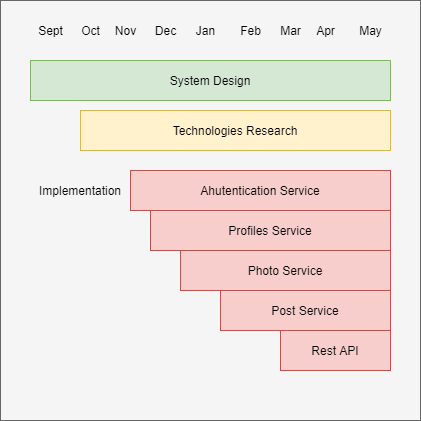
\includegraphics[width=120mm,scale=1]{img/metodology/gueneral-gant.png}
		\caption{Methodology- Project Gueneral Gant Chart.}
		\label{methodology:stages}
	\end{center}
	
\end{figure}

\paragraph{System Design}

We create a simple design of the system at the start. This defines, in a general way, the main components of the system. This was a quick process, and the design was always subject to updates.
To design the system, first, the requirements where set. Then the design was done following them.


\begin{itemize}
	\item Design the full system in a general way, understand more or less the number of services required.
	\item Define the function of each component.
	
\end{itemize}


\paragraph{Technology Research}

After we have an idea of the system, some time was spent on looking for the best technologies that will suit the application, some prototypes where design to check if they work.

\begin{itemize}
	\item Decide the main technologies to be used.
	\item	Test compatibility. 
\end{itemize}



\paragraph{ Implementation}

The implementation has been done using an iterative process. Starting from the authentication service, the system was build block by block. After one component was developed, it was tested to check that the full system works. 

On each component, we start by designing the database, the DBA, and then the main service with the endpoint to the client.

When starting to develop a new component, the full system design has to be check.


\subsection{System Development life cycle}
\indent
\indent
Each component is developed iteratively after some functionality is implemented the component is first tested locally, them docker images is created ann updated to docker hub, them the image is downloaded in the server, and the whole system is tested. The life cycle steps are below(Figure \ref{methodology:cycle}):

\begin{itemize}
	\item Build and test the component locally.
	\item Create/update a docker image and update it to the docker hub.
	\item Pull from docker hub, run the component in the network, and test.
	\item Test the full system. 
\end{itemize}


\begin{figure}
	\begin{center}
		\includegraphics[width=120mm,scale=1]{img/metodology/component-teration.png}
		\caption{Methodology- Component Iteration.}
		\label{methodology:cycle}
	\end{center}
	
\end{figure}

\subsection{Selection Criteria}
\label{sel:criteria}
\indent
\indent
We have applied the following criteria to chose the technologies used in the project.
\begin{itemize}
	
	
	\item Accessibility. Technologies must be accessible without a cost; they can be free and open-source or offer student free usage.
	\item New to us. One of the ideas of the project is to learn how to work with new technologies and learn. So we look for technologies that are not familiar to us.
	
	\item Popular and used in 
	They are professionally used. We want to learn how to use technologies that are popular and used in professional software development.
	
	\item Mature and recognized. We prefer technologies with background and maintained/developed by a recognized organization or a big open source community. Even if there are always new technologies coming out, we prefer those that are already established.
	
	\item It adapts well to the purpose need in the system.
	Simple and with resources to learn. We need to learn the technologies, so we instead chose those that are fast to learn and with many resources(tutorials and documentation) to access.
\end{itemize}

\subsection{ Testing}
\indent
\indent
Because of the time frame, we do not develop the application using automated testing. We know there are many advantages to it, but we need to trade off this feature. Some aspects that we considered to decide that automated testing is not for the project:
Most of the benefits of automated testing are long time benefits.
Automatested testing is practical another application that needs to be maintained.

Instead, based on the principle of self-motivated development, we develop the project using a test culture that relies on developers:
Each functionality needs to be tested by the developer at developing time.
Bugs found needs to be personally reported to the developer.
When integrating new components, the full system needs to be checked. 

\subsection{Security considerations for authentication}
\begin{itemize}

	\item  Feedback for password strength.
	\item  hash+ salt using bcrypt function on server and client.
	\item constant time function for compare hashed passwords.
\end{itemize}
\subsection{Tools}



\subsubsection{Integrated development environment}

\begin{itemize}

	\item  Eclipse for Java development. Solid IDE with just the right performance, we choose it because its well knows for us and free to use (\url{https://www.eclipse.org/}).
	\item  Goland, for Go development. Excellent IDE is free for students(\url{https://www.jetbrains.com/go/}). 
	\item  Visual Studio Code, general code review, and write docker images(\url{https://code.visualstudio.com/}).

\end{itemize}
\subsubsection{SHH Client}
\begin{itemize}
	
	\item  Putty, free shh client, open-source, and simple to use(\url{https://www.putty.org/}).
\end{itemize}

\subsubsection{Version Management}
\begin{itemize}
\item  Git, very popular with string community, we use the prevalent GitHub server(\url{https://git-scm.com/}). 
\item  Docker Hub, Manage containers, free for public containers (\url{https://hub.docker.com/}). 
\end{itemize}
